\documentclass{beamer}
\usepackage{graphicx}
\usepackage{listings}
\usepackage{multicol}
% \usetheme{metropolis}
\usetheme{Rochester}

\title[WebAssembly]{WebAssembly}
\author{Jakob Waibel}
\institute[Jakob Waibel]{MI7 Druck und Medien}
\date

\begin{document}

\begin{frame}
    \titlepage
\end{frame}

\begin{frame}
    \setbeamerfont{subsection in toc}{size=\small}
    \frametitle{Agenda}
    \begin{multicols}{2}
    \tableofcontents
    \end{multicols}
\end{frame}

\section{Introduction}

\begin{frame}{Motivation}
    \begin{figure}
        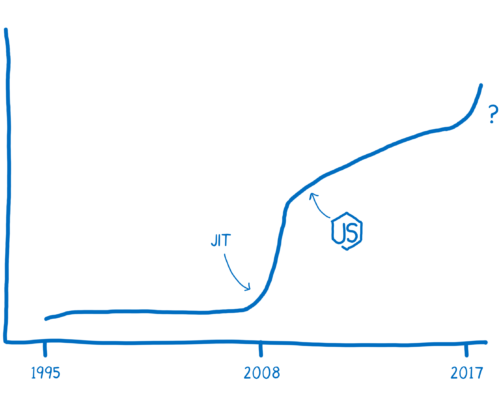
\includegraphics[width=0.7\textwidth,height=0.7\textheight]{./images/perf_history.png}
        \caption{\href{https://hacks.mozilla.org/2017/02/a-cartoon-intro-to-webassembly/}{Performance-Entwicklung im Web-Kontext}}
    \end{figure}
\end{frame}

\section{Key Concepts}

\subsection{Definition}

\begin{frame}{Definition}
    \begin{figure}
        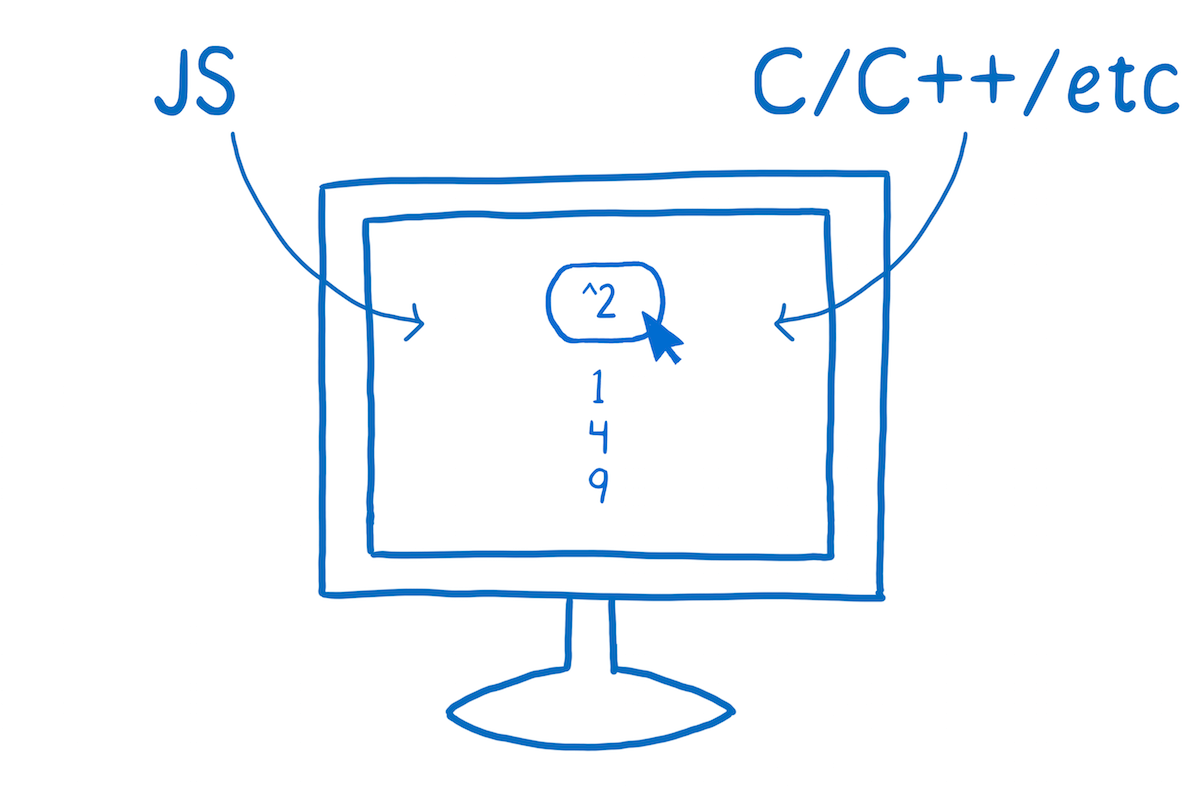
\includegraphics[scale=0.2]{./images/definition.png}
        \caption{\href{https://www.smashingmagazine.com/2017/05/abridged-cartoon-introduction-webassembly/}{Introduction to WebAssembly}}
    \end{figure}
\end{frame}

\begin{frame}{Definition}
    \begin{figure}
        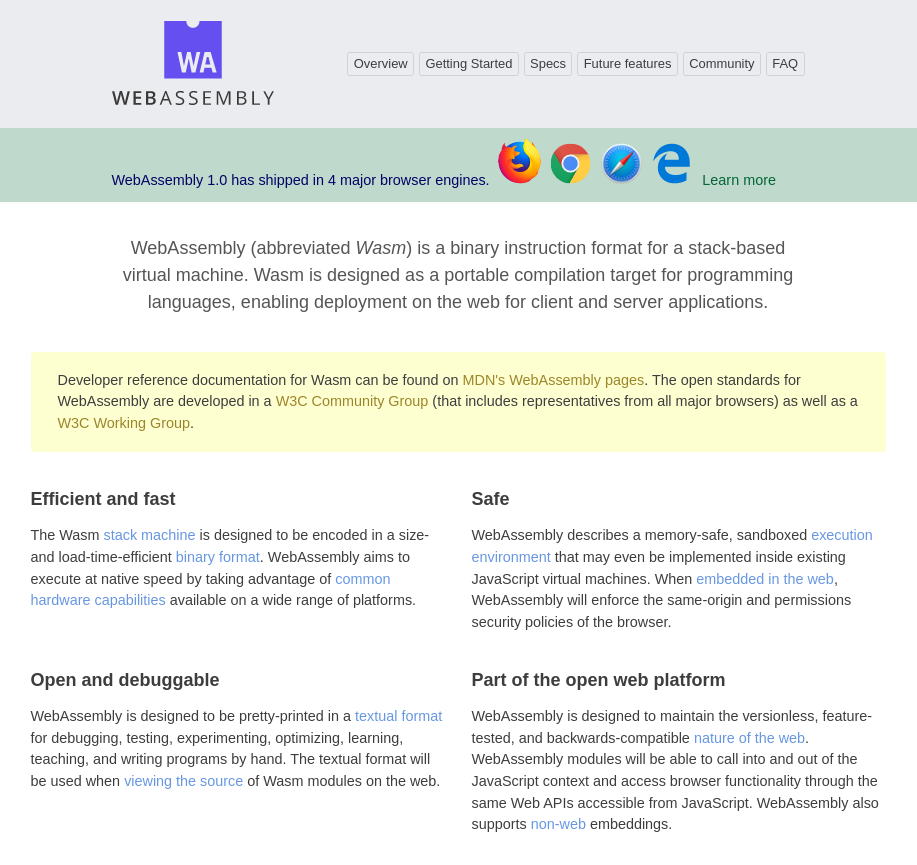
\includegraphics[scale=0.2]{./images/webassembly_org.png}
        \caption{\href{https://webassembly.org/}{webassembly.org}}
    \end{figure}
\end{frame}

\begin{frame}{Definition}
    \begin{quotation}
        "\textbf{WebAssembly} (abbreviated Wasm) is a \textbf{binary instruction format} for a \textbf{stack-based virtual machine}. Wasm is designed as a \textbf{portable compilation target} for programming languages, \textbf{enabling deployment on the web} for client and server applications."
    \end{quotation}
\end{frame}

\subsection{Binary Instruction Format}

\begin{frame}{Binary Instruction Format}
    \begin{itemize}
        \item Machine instruction format consisting of \textbf{1s and 0s} that can be directly decoded and \textbf{executed by the CPU}
        \item \textbf{Targeting different instruction set architectures} (ISA) like x86, ARM or RISC-V
        \item WASM uses \textbf{virtual instructions} for a \textbf{conceptual machine}, not a physical one
        \item Think of WASM instruction set as "intersection" of multiple ISAs that can't be mapped directly to one ISA
    \end{itemize}
\end{frame}

\subsection{Stack-Based Virtual Machine}

\begin{frame}{Stack-Based Virtual Machine}
    \begin{itemize}
        \item Virtual machine which uses stacks to perform oprations
        \item Famous stack-based VMs are the JVM (Java Virtual Machine) and the CLR (Common Language Runtime)
        \item E.g. to add two numbers in a stack-based VM, the program will push the first number to the stack, push the second and then execute some form of the special instruction add, that will pop the first two elements of the stack and replace them with their sum
        \item When the browser translates WASM to the machine code for the machine the browser is running on, it will use registers. Since the WASM specification does not specify registers, it gives the browser more flexibility to use the best register allocation for  that machine
    \end{itemize}
\end{frame}

\subsection{Portable Compilation Target}

\begin{frame}{Portable Compilation Target}
    \begin{itemize}
        \item \textbf{WASM is designed to be executable on a variety of operating systems and instruction set architectures, on the Web and off the Web}
        \item Created as an \textbf{open standard} inside the W3C WebAssembly Community Group
        \item \textbf{Requirements} for WASM execution environments:
              \begin{itemize}
                  \item 8-bit Bytes
                  \item Addressable at byte granularity
                  \item Little endian
                  \item \href{https://webassembly.org/docs/portability/}{...}
              \end{itemize}
    \end{itemize}
\end{frame}

\subsection{Deployment on the Web Platform}

\begin{frame}{Deployment on the Web Platform}
    \begin{itemize}
        \item The \textbf{web platform} can be described in two parts
              \begin{itemize}
                  \item A \textbf{VM/Engine} that runs the code, e.g. V8 or SpiderMonkey
                  \item A set of \textbf{Web APIs} that can be called to control browser/device functionality (DOM, WebGL, Web Audio API etc.)
              \end{itemize}
        \item In the past, only JS could be executed in the browser as it was good enough. Today some performance problems occur as we have to run intensive programs like 3D games, VR and AR etc.
        \item The VM can now load an run two types of code: \textbf{JavaScript and WebAssembly}
        \item The different code types \textbf{can call each other}. The WebAssembly JavaScript API wraps exported JavaScript code with JavaScript functions that can be called normally and WebAssembly code can import and synchronously call normal JavaScript functions.
    \end{itemize}
\end{frame}

\begin{frame}{Definition}
    \begin{quotation}
        "\textbf{WebAssembly} (abbreviated Wasm) is a \textbf{binary instruction format} for a \textbf{stack-based virtual machine}. Wasm is designed as a \textbf{portable compilation target} for programming languages, \textbf{enabling deployment on the web} for client and server applications."
    \end{quotation}
\end{frame}

\subsection{Use Cases}

\begin{frame}{Use Cases}
    Considered by the W3C as now more feasable inside the browser:
    \begin{itemize}
        \item Better execution for languages and toolkits that are currently cross-compiled to the Web
        \item VR and AR
        \item Platform simulation / emulation (DOSBox, QEMU, …)
        \item Remote desktop
        \item Games
        \item Cloud IDEs
        \item \href{https://webassembly.org/docs/use-cases/}{...}
    \end{itemize}
    Outside the browser:
    \begin{itemize}
        \item Server-side applications
        \item Game distribution services
        \item Parallel computation across multiple nodes
    \end{itemize}
\end{frame}

\begin{frame}
    Projects using WebAssembly right now:
    \begin{itemize}
        \item Blazor
        \item Autocad
        \item Figma
        \item Jitsi for virtual backgrounds
        \item Zoom for video encoding
        \item \href{https://wasm.continuation-labs.com/d3demo/}{D3wasm}
        \item ...
    \end{itemize}
\end{frame}

\subsection{WebAssembly Text}
% Talk about S-expressions, import, exports, types, globals and shared memory and talk about why it might be not that relevant for the "normal" webdev
\begin{frame}[fragile]{WebAssembly Text}
    \begin{itemize}
        \item Textual representation of the binary format to allow reading and editing by humans
        \item Designed to be exposed in text editors, browser developer tools, etc.
    \end{itemize}
    \begin{lstlisting}[language=Lisp,basicstyle=\scriptsize]
(module
  (func $add (param $lhs i32) (param $rhs i32) (result i32)
    local.get $lhs
    local.get $rhs
    i32.add)
  (export "add" (func $add))
)
    \end{lstlisting}
    \begin{itemize}
        \item .wat files can be compiled to .wasm using the WebAssembly Binary Toolkit (WABT)
        \item For more information, consider visiting the \href{https://developer.mozilla.org/en-US/docs/WebAssembly/Understanding_the_text_format}{MDN Web Docs}
    \end{itemize}
\end{frame}

\section{Demo}

\begin{frame}{Demo - Prerequisites}
    Disclaimer: This Demo is using the \href{https://go.dev/}{Go} programming language. You don't need any knowledge about Go to follow this Demo. Furthermore, I am using Linux! I can't guarantee, nor do I care, that it works on your Windows machine.

    Installing the Go programming language:
    \begin{itemize}
        \item Please follow \underline{\href{https://go.dev/doc/install}{this}} tutorial
    \end{itemize}

\end{frame}

\begin{frame}[fragile]{Demo - File structure}

    \begin{lstlisting}[language=Bash,basicstyle=\scriptsize]
go/
    assets/
        index.html
        main.wasm
        wasm_exec.js
    cmd/
        server/
            main.go
        wasm/
            main.go
    \end{lstlisting}
\end{frame}

\begin{frame}[fragile]{Demo - main.go}
    \begin{lstlisting}[language=Go,basicstyle=\scriptsize]
package main

import "fmt"

func main() {
	fmt.Println("Hello World!")
}

    \end{lstlisting}
\end{frame}

\subsection{Compilation}

\begin{frame}[fragile]{Demo - Compilation}
    To compile your main.go to a WebAssembly main.wasm file, execute the following command in the wasm directory:

    \begin{lstlisting}[language=Bash,basicstyle=\scriptsize]
$ GOOS=js GOARCH=wasm go build -o  ../../assets/main.wasm
    \end{lstlisting}

    You should now be able to locate a \lstinline{main.wasm} file inside your \lstinline{assets} folder.
\end{frame}

\begin{frame}[fragile]{Demo - JavaScript Glue Code}
    Some JavaScript code is needed to import the WebAssembly Module we just created in the Browser. Fortunately, this code comes with every Go installation. So just go ahead and copy the file into your \lstinline{assets} directory:

    \begin{lstlisting}[language=Bash,basicstyle=\scriptsize]
$ cp "$(go env GOROOT)/misc/wasm/wasm_exec.js" .
\end{lstlisting}
\end{frame}

% The WebAssembly.instantiateStreaming() function compiles and instantiates a WebAssembly module directly from a 
% streamed underlying source. This is the most efficient, optimized way to load wasm code.
\begin{frame}[fragile]{Demo - index.html}
    \begin{lstlisting}[language=html,basicstyle=\scriptsize]
<html>
    <head>
        <meta charset="utf-8"/>
        <script src="wasm_exec.js"></script>
        <script>
            const go = new Go();

            WebAssembly.instantiateStreaming(
                fetch("main.wasm"), go.importObject
            )
            .then((result) => {
                go.run(result.instance);
            })
        </script>
    </head>
    <body></body>
</html>
\end{lstlisting}
\end{frame}

\begin{frame}[fragile]{Demo - cmd/server/main.go}
    \begin{lstlisting}[language=html,basicstyle=\scriptsize]
package main

import (
	"fmt"
	"net/http"
)

func main() {
    err := http.ListenAndServe(
        ":9090", 
        http.FileServer(http.Dir("../../assets"))
    )
    if err != nil {
	fmt.Println("Failed to start server", err)
	return
    }
}

    \end{lstlisting}
\end{frame}

\subsection{Execution}

% Show rust demo as well
\begin{frame}[fragile]{Demo - Execution}
    Now you can run your server and inspect the outcome. Make sure you are in the \lstinline{server} directory, when executing this command:
    \begin{lstlisting}[language=bash,basicstyle=\scriptsize]
$ go run main.go
\end{lstlisting}

    Now you should be able to inspect the result in your browser:
    \begin{figure}
        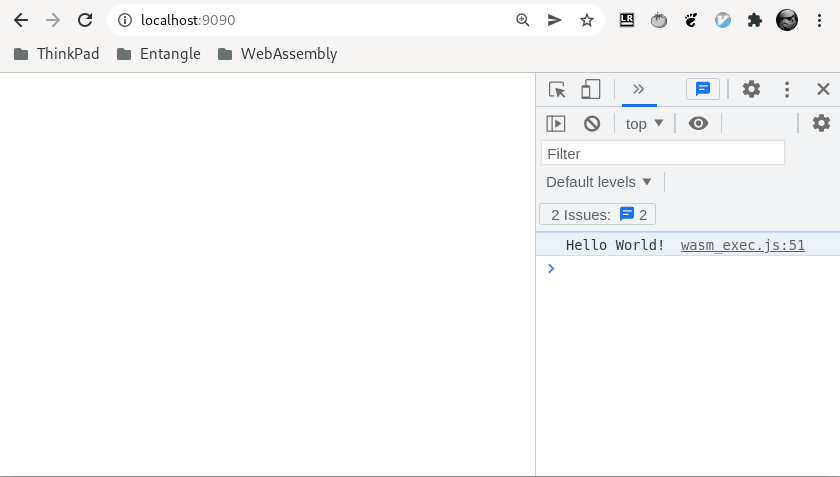
\includegraphics[scale=0.3]{./images/demo.png}
        \caption{\href{https://hacks.mozilla.org/2017/02/a-cartoon-intro-to-webassembly/}{Performance-Entwicklung im Web-Kontext}}
    \end{figure}
\end{frame}

\subsection{Exports}

\begin{frame}{Demo - Exports}
    Essentially same procedure. Just exchange the contents of the following files:
    \begin{figure}
        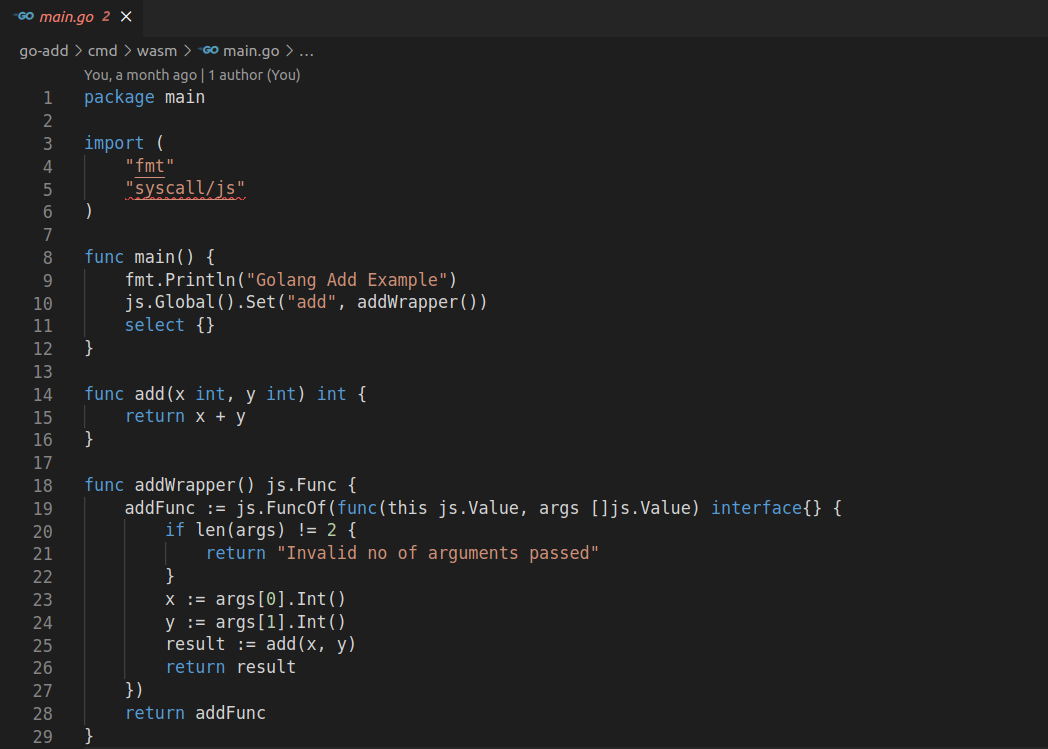
\includegraphics[scale=0.2]{./images/main.png}
        \caption{main.go}
    \end{figure}

\end{frame}

\begin{frame}{Demo - Exports}
    \begin{figure}
        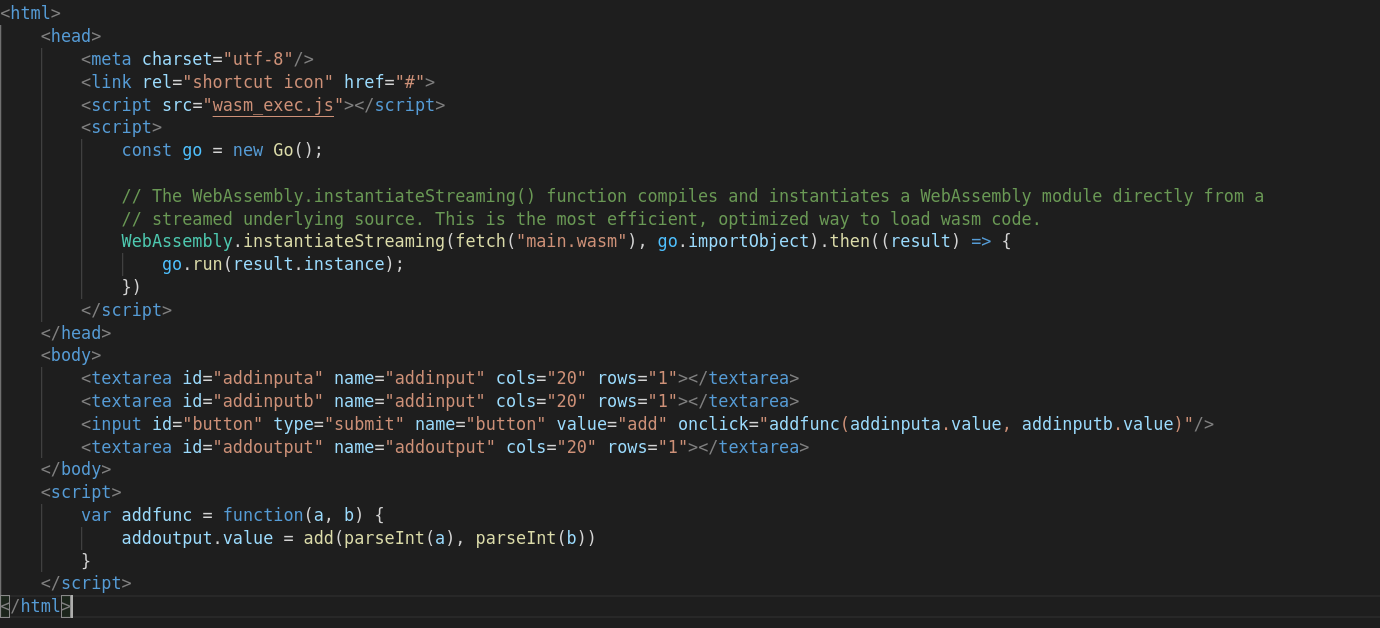
\includegraphics[scale=0.2]{./images/index.png}
        \caption{index.html}
    \end{figure}

\end{frame}

\subsection{Imports}

\begin{frame}{Demo - Imports}
    Essentially same procedure. This time, exchange the contents of the following files:
    \begin{figure}
        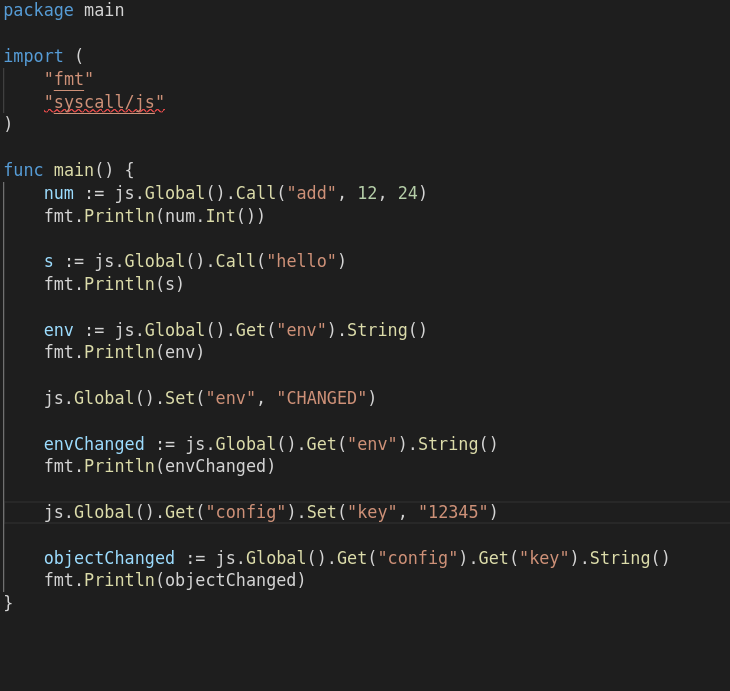
\includegraphics[scale=0.2]{./images/maingo.png}
        \caption{main.go}
    \end{figure}

\end{frame}

\begin{frame}{Demo - Imports}
    \begin{figure}
        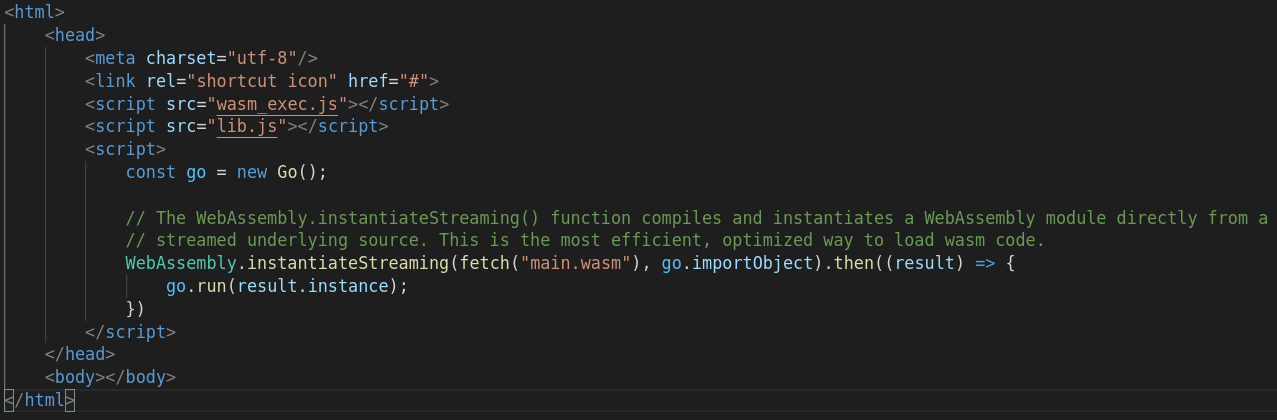
\includegraphics[scale=0.25]{./images/jsindex.png}
        \caption{index.html}
    \end{figure}

\end{frame}

\begin{frame}{Demo - Imports}
    \begin{figure}
        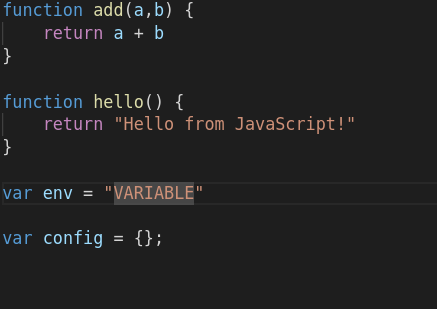
\includegraphics[scale=0.4]{./images/libjs.png}
        \caption{lib.js}
    \end{figure}

\end{frame}

\begin{frame}{Additional Information}
    \begin{itemize}
        \item Linear Memory - Continuous buffer of unsigned bytes that can be read from and stored into by both Wasm and Javascript
        \item Dom Manipulation - The syscall/js package can also be used to interact with the DOM. WASM can not directly interact with the DOM! It has to call JS!
        \item E.g. Rust is using wasm-bindgen to achieve the same as Go with syscall/js, AssemblyScript provides those features out of the box...
        \item WASM function only support ints and floats. To work with other data types, linear memory can be used
    \end{itemize}
\end{frame}

% Add terminlogy but don't talk about it in the presentation. It should be clear after the Demo
\begin{frame}{Terminology}
    \begin{itemize}
        \item \textbf{Module}: WebAssembly Binary that has beed compiled into executable machine code. A Module is stateless and thus, like a Blob, can be explicitly shared between windows and workers. Module declares imports just like an ES2015 module.
        \item \textbf{Memory}: A resizable ArrayBuffer that contains the linear array of bytes read and written by WebAssembly’s low-level memory access instructions.
        \item \textbf{Table}: A resizable typed array of references (e.g. to functions) that could not otherwise be stored as raw bytes in Memory (for safety and portability reasons).
        \item \textbf{Instance}: A Module paired with all the state it uses at runtime including a Memory, Table, and set of imported values. An Instance is like an ES2015 module that has been loaded into a particular global with a particular set of imports.
    \end{itemize}
\end{frame}

\section{Evaluation}

\begin{frame}{Evaluation}
    \begin{figure}
        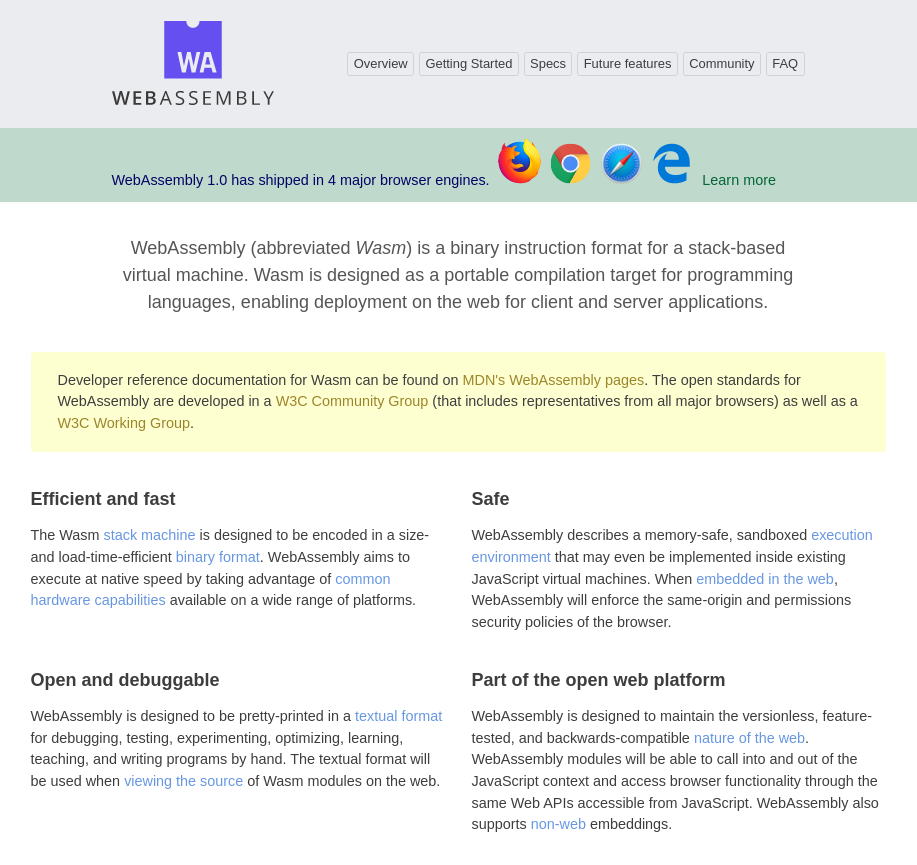
\includegraphics[scale=0.2]{./images/webassembly_org.png}
        \caption{\href{https://webassembly.org/}{webassembly.org}}
    \end{figure}
\end{frame}

% Comparison between JS and WASM. Also talk about asm.js
\begin{frame}{Efficient and fast}
    \begin{figure}
        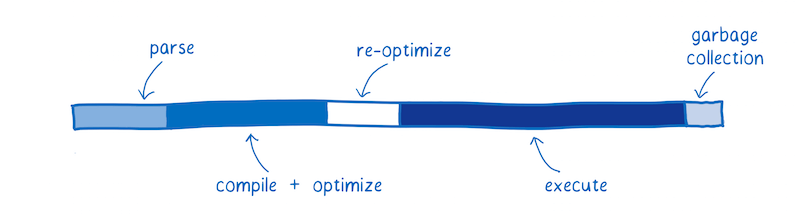
\includegraphics[scale=0.3]{./images/javascriptgraph.png}
        \caption{\href{https://www.smashingmagazine.com/2017/05/abridged-cartoon-introduction-webassembly/}{Time distribution when running JavaScript}}
    \end{figure}
    \begin{figure}
        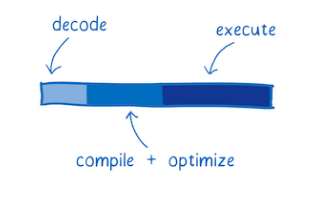
\includegraphics[scale=0.4]{./images/wasmgraph.png}
        \caption{\href{https://www.smashingmagazine.com/2017/05/abridged-cartoon-introduction-webassembly/}{Time distribution when running WebAssembly}}
    \end{figure}
\end{frame}

\subsection{Fetching} 

\begin{frame}{Efficient and fast - Fetching}
    \begin{figure}
        
\includegraphics[scale=0.2]{./images/file.jpg}
        \caption{\href{https://icon-library.com/icon/download-icon-file-4.html}{Fetch}}
    \end{figure}
    \begin{itemize}
        \item Fetching (not on diagram): Fetching file from server. WASM more compact as it's designed that way. WASM is even smaller than a gzipped JavaScript file
    \end{itemize}
\end{frame}

\subsection{Parsing}

\begin{frame}{Efficient and fast - Parsing}
    \begin{figure}
        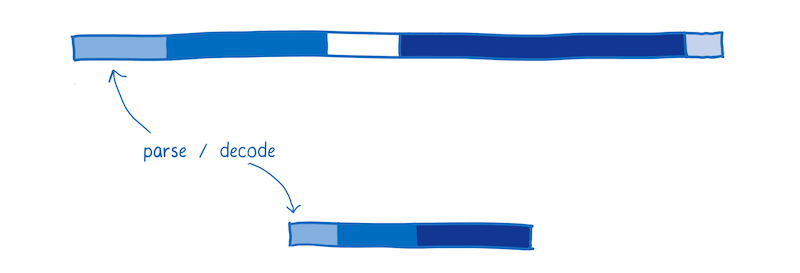
\includegraphics[scale=0.2]{./images/pasedecode.png}
        \caption{\href{https://www.smashingmagazine.com/2017/05/abridged-cartoon-introduction-webassembly/}{Parse}}
    \end{figure}
    \begin{itemize}
        \item Javascript gets parsed to AST (lazy). From there the JS code is parsed to intermediate representation (byte code). WASM does not need this step because we already get bytecode. WASM bytecode just needs to be decoded and validated
    \end{itemize}
\end{frame}

\subsection{Compilation + Optimization}

\begin{frame}{Efficient and fast - Compilation + Optimization}
    \begin{figure}
        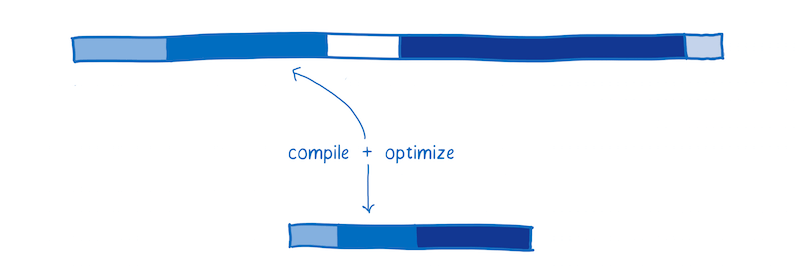
\includegraphics[scale=0.2]{./images/copyoptimize.png}
        \caption{\href{https://www.smashingmagazine.com/2017/05/abridged-cartoon-introduction-webassembly/}{Compilation}}
    \end{figure}
    \begin{itemize}
        \item JS is compiled during the execution of the code. Because types are dynamic, multiple versions of the same code may need to be compiled.
        \item WebAssembly saves time with regards to:
              \begin{itemize}
                  \item Don't need to figure out used types
                  \item Ahead of time optimizations in e.g. LLVM
              \end{itemize}
    \end{itemize}
\end{frame}

\subsection{Reoptimization}

\begin{frame}{Efficient and fast - Reoptimizaion}
    \begin{figure}
        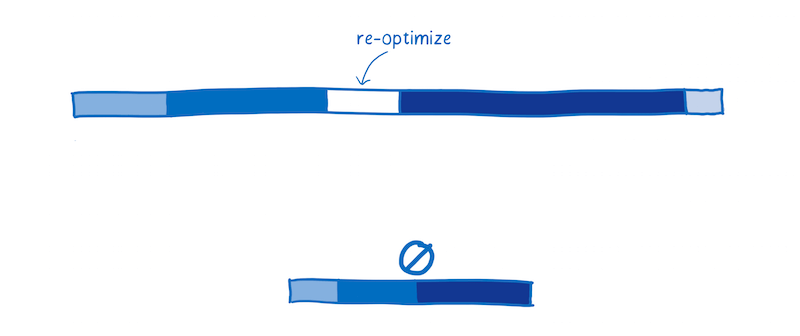
\includegraphics[scale=0.2]{./images/re-optimize.png}
        \caption{\href{https://www.smashingmagazine.com/2017/05/abridged-cartoon-introduction-webassembly/}{Reoptimization}}
    \end{figure}
    \begin{itemize}
        \item JIT assumptions about the code may be incorrect and a rollback is needed
        \item Deoptimization happens when variables in a loop are different than they were in previous iterations
        \item WebAssembly does not need reoptimization since types are explicit an no assumptions about them are necessary during runtime
    \end{itemize}
\end{frame}

\subsection{Execution}

\begin{frame}{Effecient and fast - Execution}
    \begin{figure}
        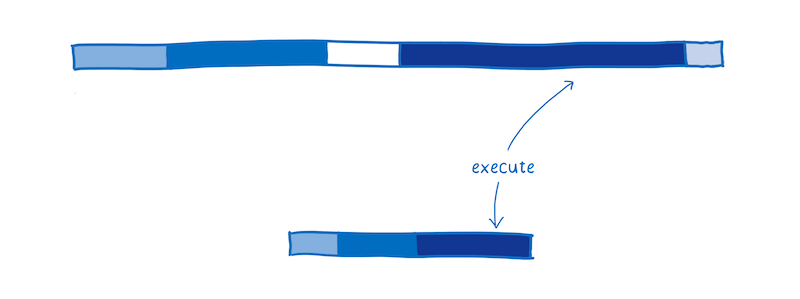
\includegraphics[scale=0.2]{./images/execution.png}
        \caption{\href{https://www.smashingmagazine.com/2017/05/abridged-cartoon-introduction-webassembly/}{Execution}}
    \end{figure}
    \begin{itemize}
        \item Most developers don't know about JIT internals, so writing performant JS code is hard
        \item WASM is designed to be a compiler target, not a human readable language. Instruction set is optimized for machines
        \item Speedup up to 800\%
        \item WebAssembly executes at "native speed"
    \end{itemize}
\end{frame}

\subsection{Garbage Collection}

\begin{frame}{Effecient and fast - Garbage Collection}
    \begin{figure}
        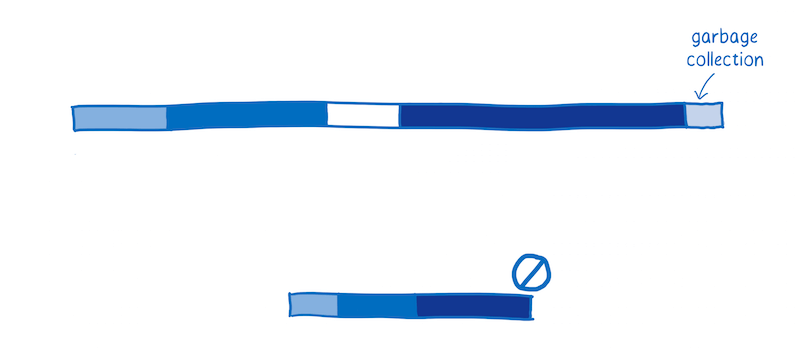
\includegraphics[scale=0.2]{./images/garbage.png}
        \caption{\href{https://www.smashingmagazine.com/2017/05/abridged-cartoon-introduction-webassembly/}{Garbage Collection}}
    \end{figure}
    \begin{itemize}
        \item JavaScript uses garbage collector to clear unused variables from memory
        \item Not knowing when a garbage collector works can lead to unpredictable performance
        \item So far, WebAssembly does not support garbage collection
    \end{itemize}
\end{frame}

\begin{frame}{Evaluation}
    \begin{figure}
        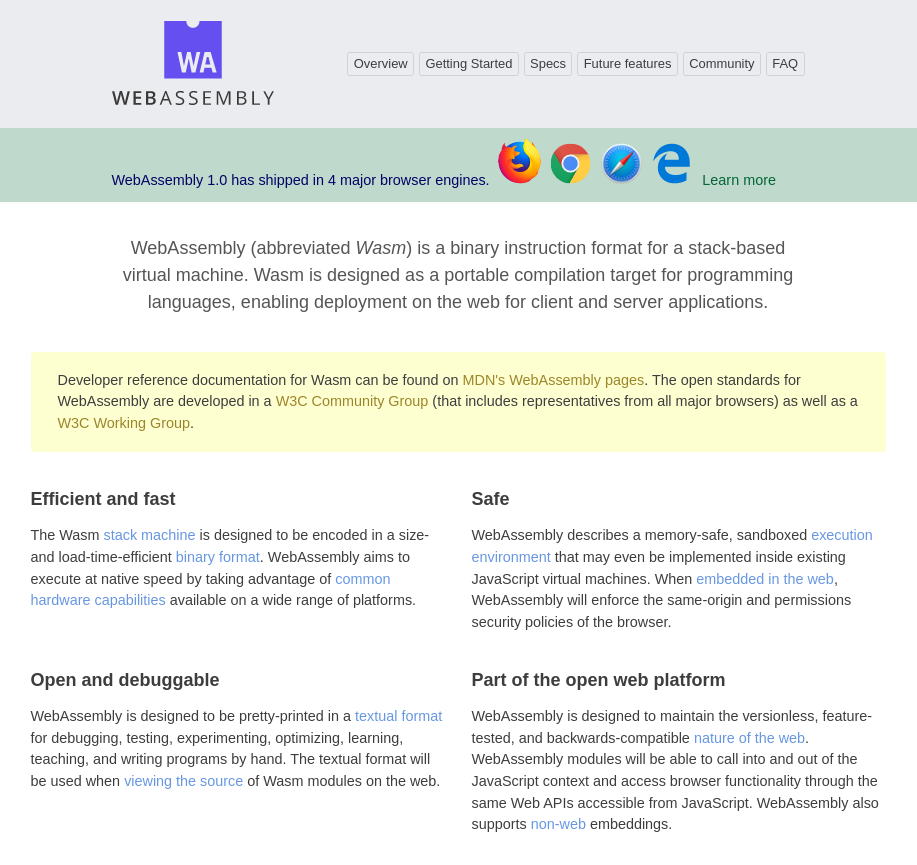
\includegraphics[scale=0.2]{./images/webassembly_org.png}
        \caption{\href{https://webassembly.org/}{webassembly.org}}
    \end{figure}
\end{frame}

% Hier fehlt eine Komponente: WASI, damit wir das richtig realisieren können. Trotz dessen beleuchten wir erst die Security und diese Grafik kann dies hervorragend beleuchten.
% \item When the operating system gets asked some input or output, it needs to determine if one is allowed the information $\rightarrow$ Ownership and Groups
% \item Protects users from each other and was useful back in time when systems were multi-user systems
% \item Nowadays it's actually more important to protect the user from itself, since most systems are single user systems
% \item We are pulling in so much third party code that whe need to control over what it can do $rightarrow$ Sandboxing
% \item Can't directly talk to the OS. Instead create a sandbox, we lock the program in and expose some functions to it with just the allowed functionality
% \item Isn't automatically secure, since the host still can grant full permissions which would be no better than the first time

\section{Security}

\begin{frame}{Security}
    \begin{figure}
        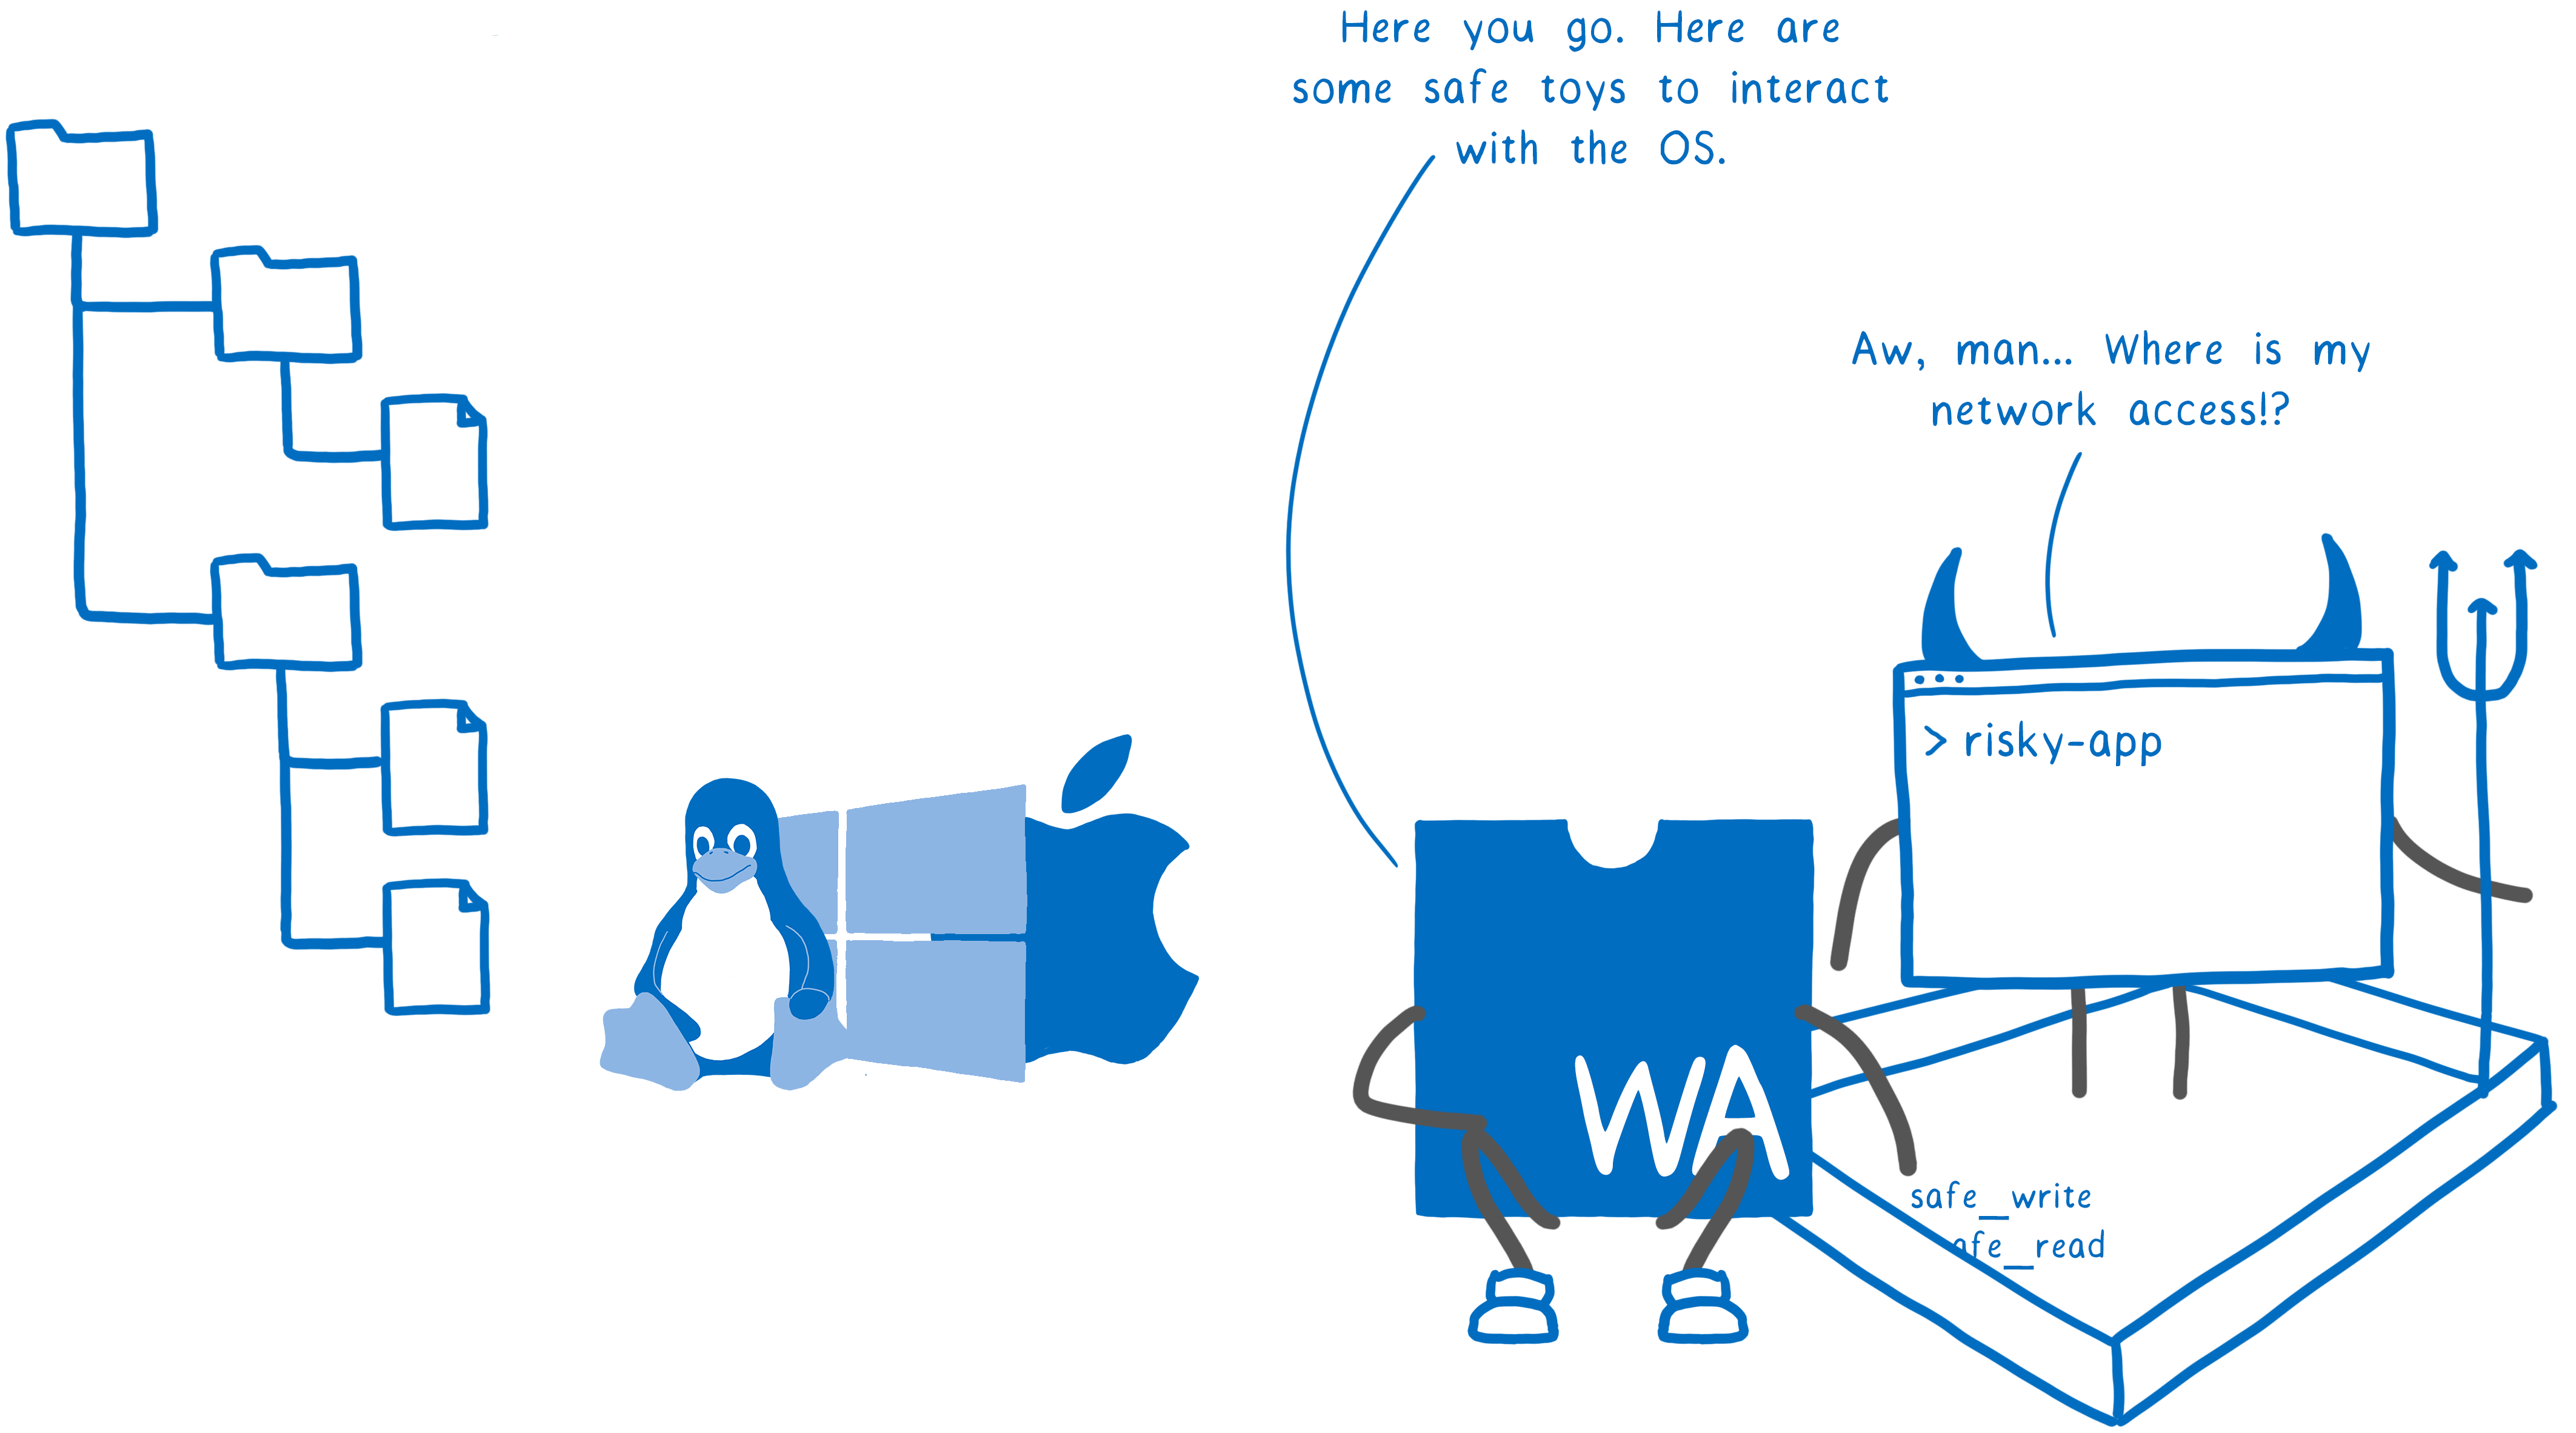
\includegraphics[scale=0.07]{./images/sandbox.png}
        \caption{\href{https://hacks.mozilla.org/2019/03/standardizing-wasi-a-webassembly-system-interface/}{Sandboxing}}
    \end{figure}
\end{frame}

% \item In normal OS, if code needs to open file, it calls the open function containing a string with the path to the file. This succeeds if the user has necessary permissions. 
% \item Instead if you call a function interacting with the files in WASI, you have to pass a file descriptor, which has permissions attached to it. This way you can't randomly open a file. Instead the code can only operate in the directory it was given.
% \item So the runtime passes in the file descriptors that an app can use at the top level code. The code itself can then propagate those file descriptors through the rest of the modules needed (Insert cude picture here)
\begin{frame}{Security}
    \begin{figure}
        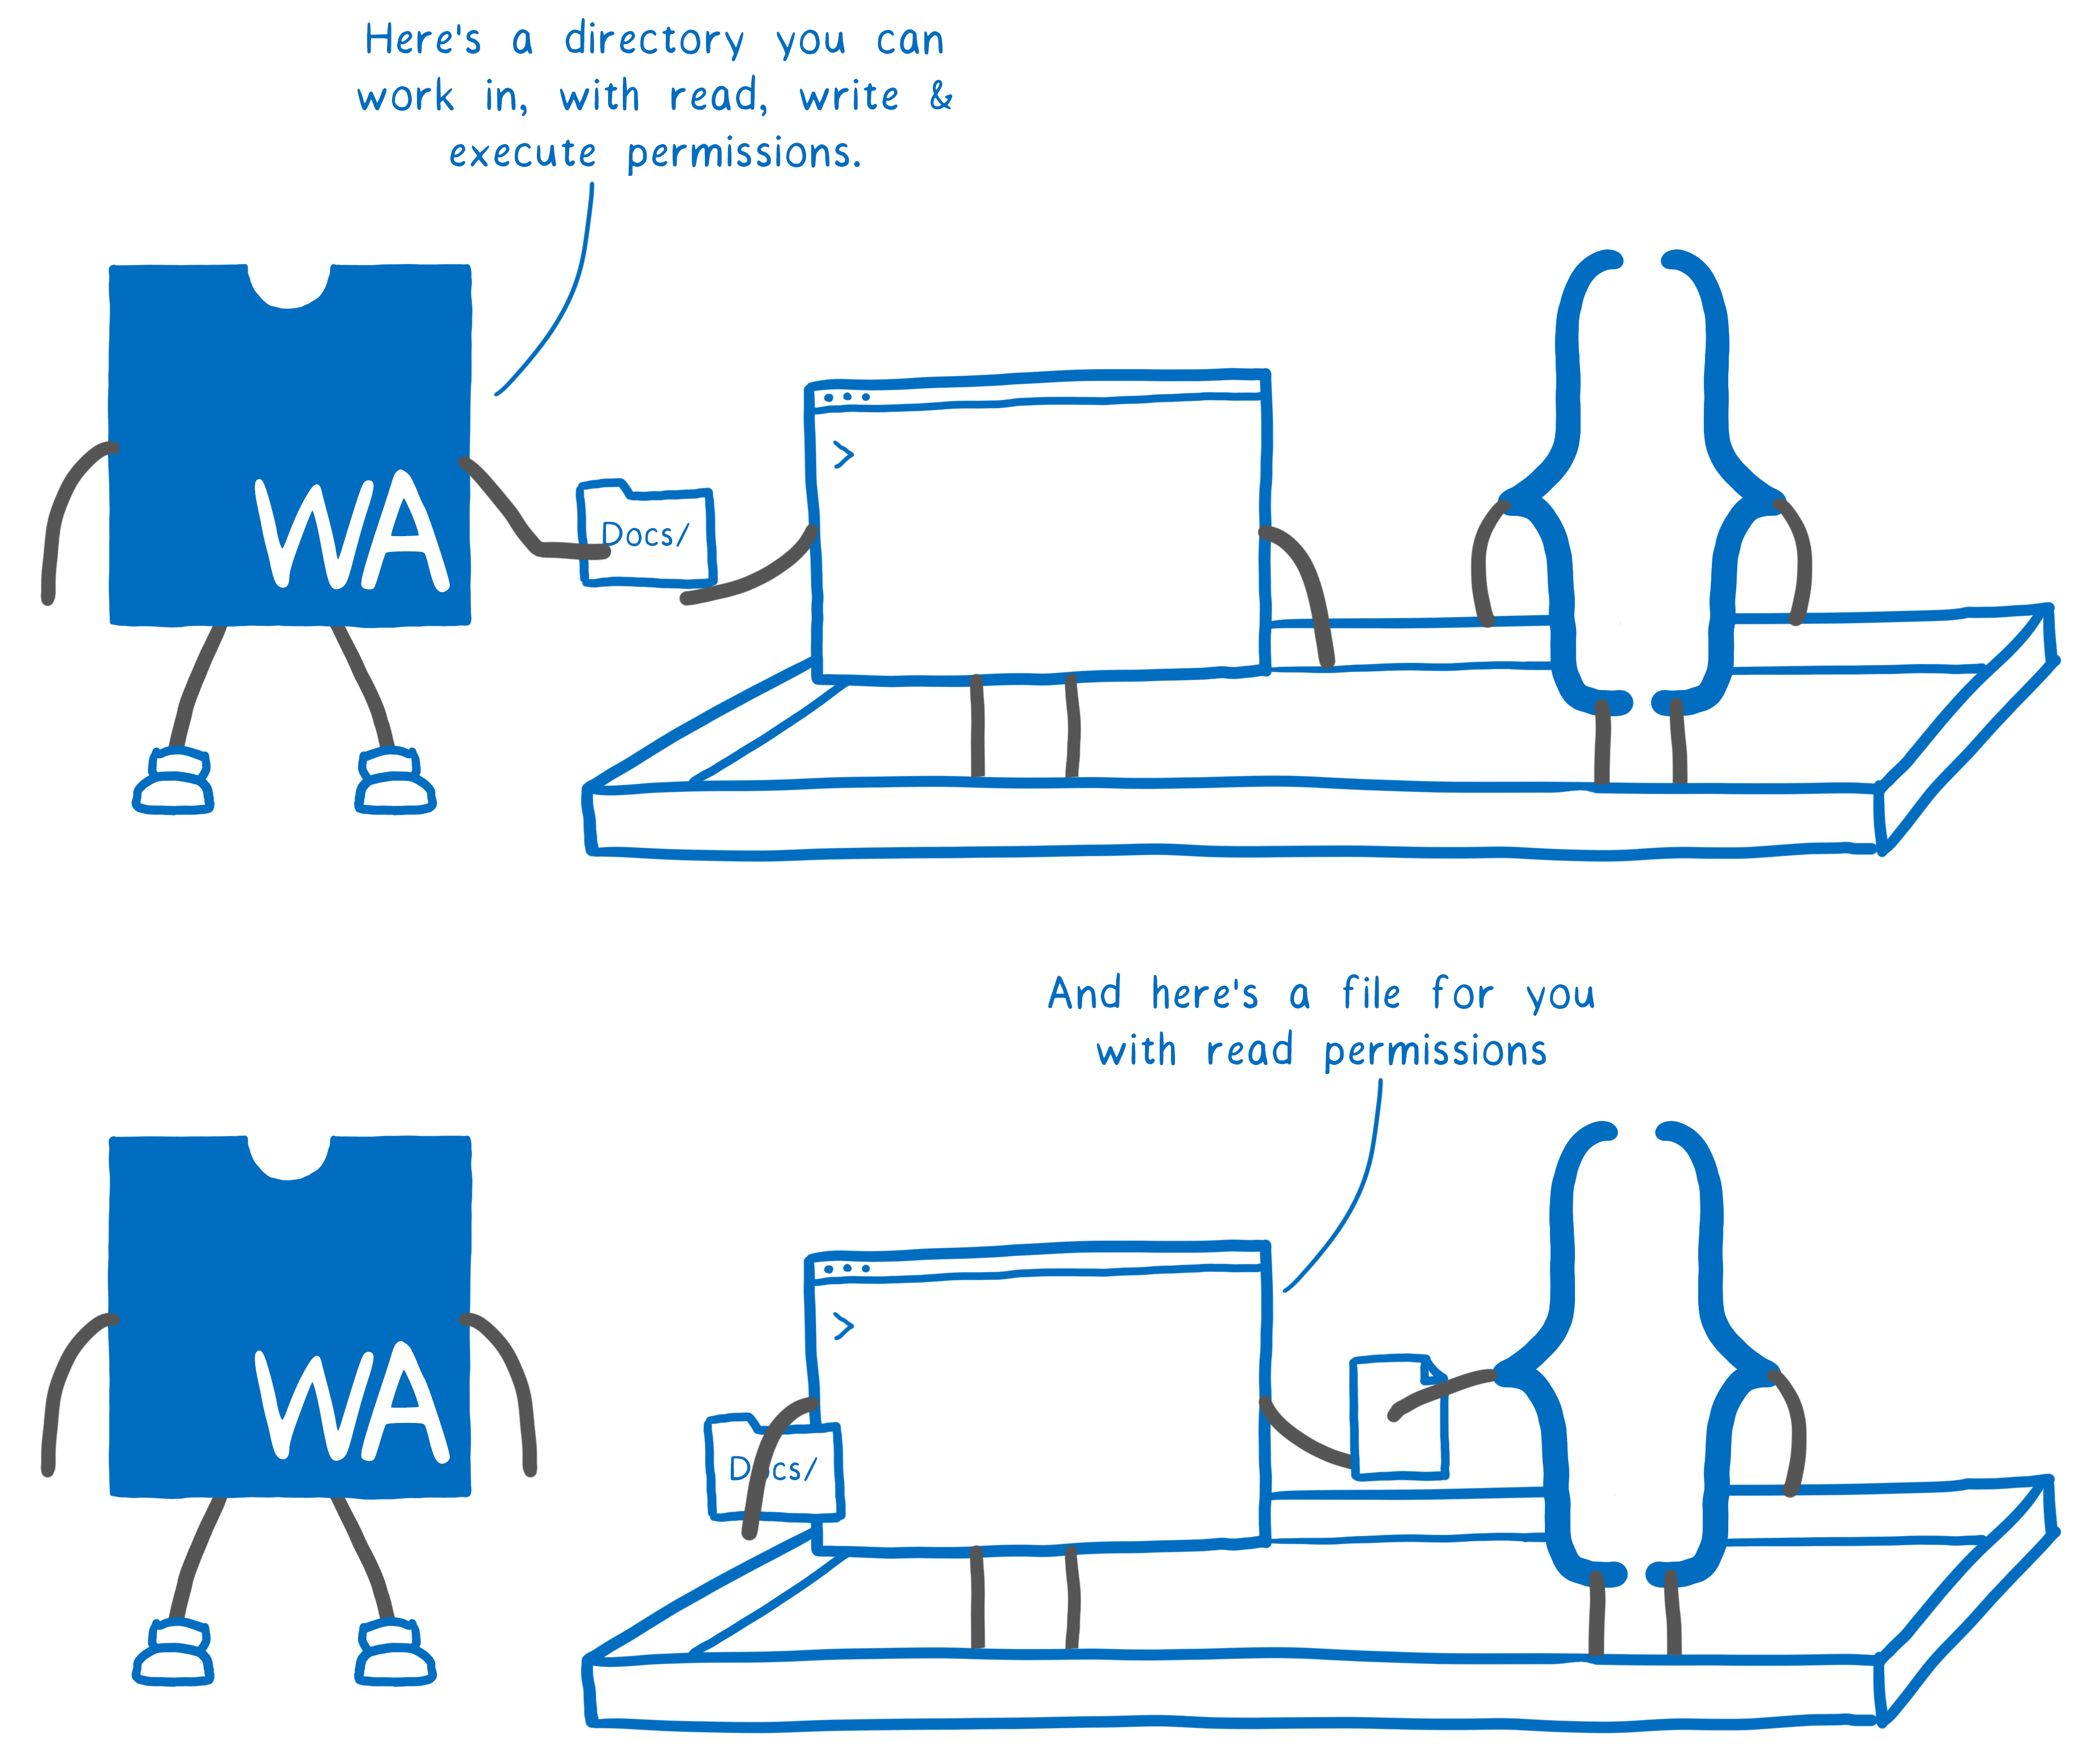
\includegraphics[scale=0.06]{./images/file.png}
        \caption{\href{https://hacks.mozilla.org/2019/03/standardizing-wasi-a-webassembly-system-interface/}{File Descriptor}}
    \end{figure}
\end{frame}

\begin{frame}{Security}
    \begin{itemize}
        \item Sandboxing as a more modern way to handle access rights
        \item Force same-origin and permission security of the browser
        \item Control-Flow-Integrity
        \item Eliminate dangerous features while maintaining compatibility with C/C++
              \begin{itemize}
                  \item Function calls must specify index of target to a valid entry in the function index space or table index space
                  \item Indirect function calls are subject to a type signature check at runtime
                  \item Protected call stack that is invulnerable to buffer overflows
                  \item Branches must point to valid destinations within the enclosing function
              \end{itemize}
        \item Memory Safety
            \begin{itemize}
                \item Variables are stored in index space, are fixed-size and addressed by index. CFI and protected call stacks prevent direct code injection attacks
                \item Unsafe pointer semantic removed. References to invalid indexes in any index space cause validation error
            \end{itemize}
    \end{itemize}
\end{frame}

\begin{frame}{Security - Attack Surface}
    \begin{itemize}
        \item Hijack the control flow of a module using code reuse attacks against indirect calls
        \item Race conditions - time of check to time of use vulnerabilities
        \item Side Channel Attacks like \href{https://github.com/tc39/ecmascript_sharedmem/blob/master/issues/TimingAttack.md}{timing attacks} against modules
        \item Probably some more...
    \end{itemize}
\end{frame}

% Lucet is deprecated for wasmtime
% Add a bit more theory
\section{Advanced Concepts}

\subsection{WebAssembly Runtimes}

\begin{frame}{WebAssembly Runtimes}
    \begin{itemize}
        \item Goal: Run WebAssembly outside of the browser
        \item Wasmer - lightweight containers that run everywhere
        \item Wasmtime - standalone JIT style runtime based on cranelift
        \item WebAssembly Micro Runtime (WAMR)
    \end{itemize}
\end{frame}

% Show wasmer demo as well
\begin{frame}[fragile]{Demo - wasmtime}
    \textbf{Install Rust:}
    \begin{lstlisting}[language=bash,basicstyle=\scriptsize]
$ curl --proto '=https' --tlsv1.2 -sSf https://sh.rustup.rs | sh
    \end{lstlisting}

    \textbf{Install wasmtime:}
    \begin{lstlisting}[language=bash,basicstyle=\scriptsize]
$ curl https://wasmtime.dev/install.sh -sSf | bash
    \end{lstlisting}

    \textbf{Add WebAssembly target to Rust:}
    \begin{lstlisting}[language=bash,basicstyle=\scriptsize]
$ rustup target add wasm32-wasi
    \end{lstlisting}

    \textbf{Compile to WebAssembly:}
    \begin{lstlisting}[language=bash,basicstyle=\scriptsize]
$ rustc main.rs --target wasm32-wasi
    \end{lstlisting}

    \textbf{Execute:}
    \begin{lstlisting}[language=bash,basicstyle=\scriptsize]
$ wasmtime main.wasm
Hello World!
    \end{lstlisting}
\end{frame}

\subsection{WebAssembly System Interface - WASI}

\begin{frame}{WebAssembly Sytem Interface - WASI}
    \begin{quotation}
        "Developers are starting to push WebAssembly beyond the browser [...]. Code outside of a browser needs a way to talk to the system [...]. And the WebAssembly platform doesn’t have that yet." - Lin Clark
    \end{quotation}
\end{frame}

% WASI - read Article
% Use preopened directories as root (based on libpreopen)
\begin{frame}{WebAssembly System Interface - WASI}
\begin{itemize} 
    \item Interact with system using syscalls
    \item Normally, the standard library of a programming language provides said system interface which is os-dependent
    \item E.g. \lstinline{prinft} being compiled for a Windows machine could use the Windows API to interact with the machine. If it's being compiled for Mac or Linux, POSIX will be used
    \item With WASM you don't know which operating system you're targeting even when you're compiling. So you can't use any single OS system interface 
    \item Portability and Security with Sandboxing
\end{itemize}
\end{frame}

% Hier fehlt eine Komponente: WASI, damit wir das richtig realisieren können. Trotz dessen beleuchten wir erst die Security und diese Grafik kann dies hervorragend beleuchten.
% \item When the operating system gets asked some input or output, it needs to determine if one is allowed the information $\rightarrow$ Ownership and Groups
% \item Protects users from each other and was useful back in time when systems were multi-user systems
% \item Nowadays it's actually more important to protect the user from itself, since most systems are single user systems
% \item We are pulling in so much third party code that whe need to control over what it can do $rightarrow$ Sandboxing
% \item Can't directly talk to the OS. Instead create a sandbox, we lock the program in and expose some functions to it with just the allowed functionality
% \item Isn't automatically secure, since the host still can grant full permissions which would be no better than the first time
\begin{frame}{WebAssembly System Interface - WASI}
    \begin{figure}
        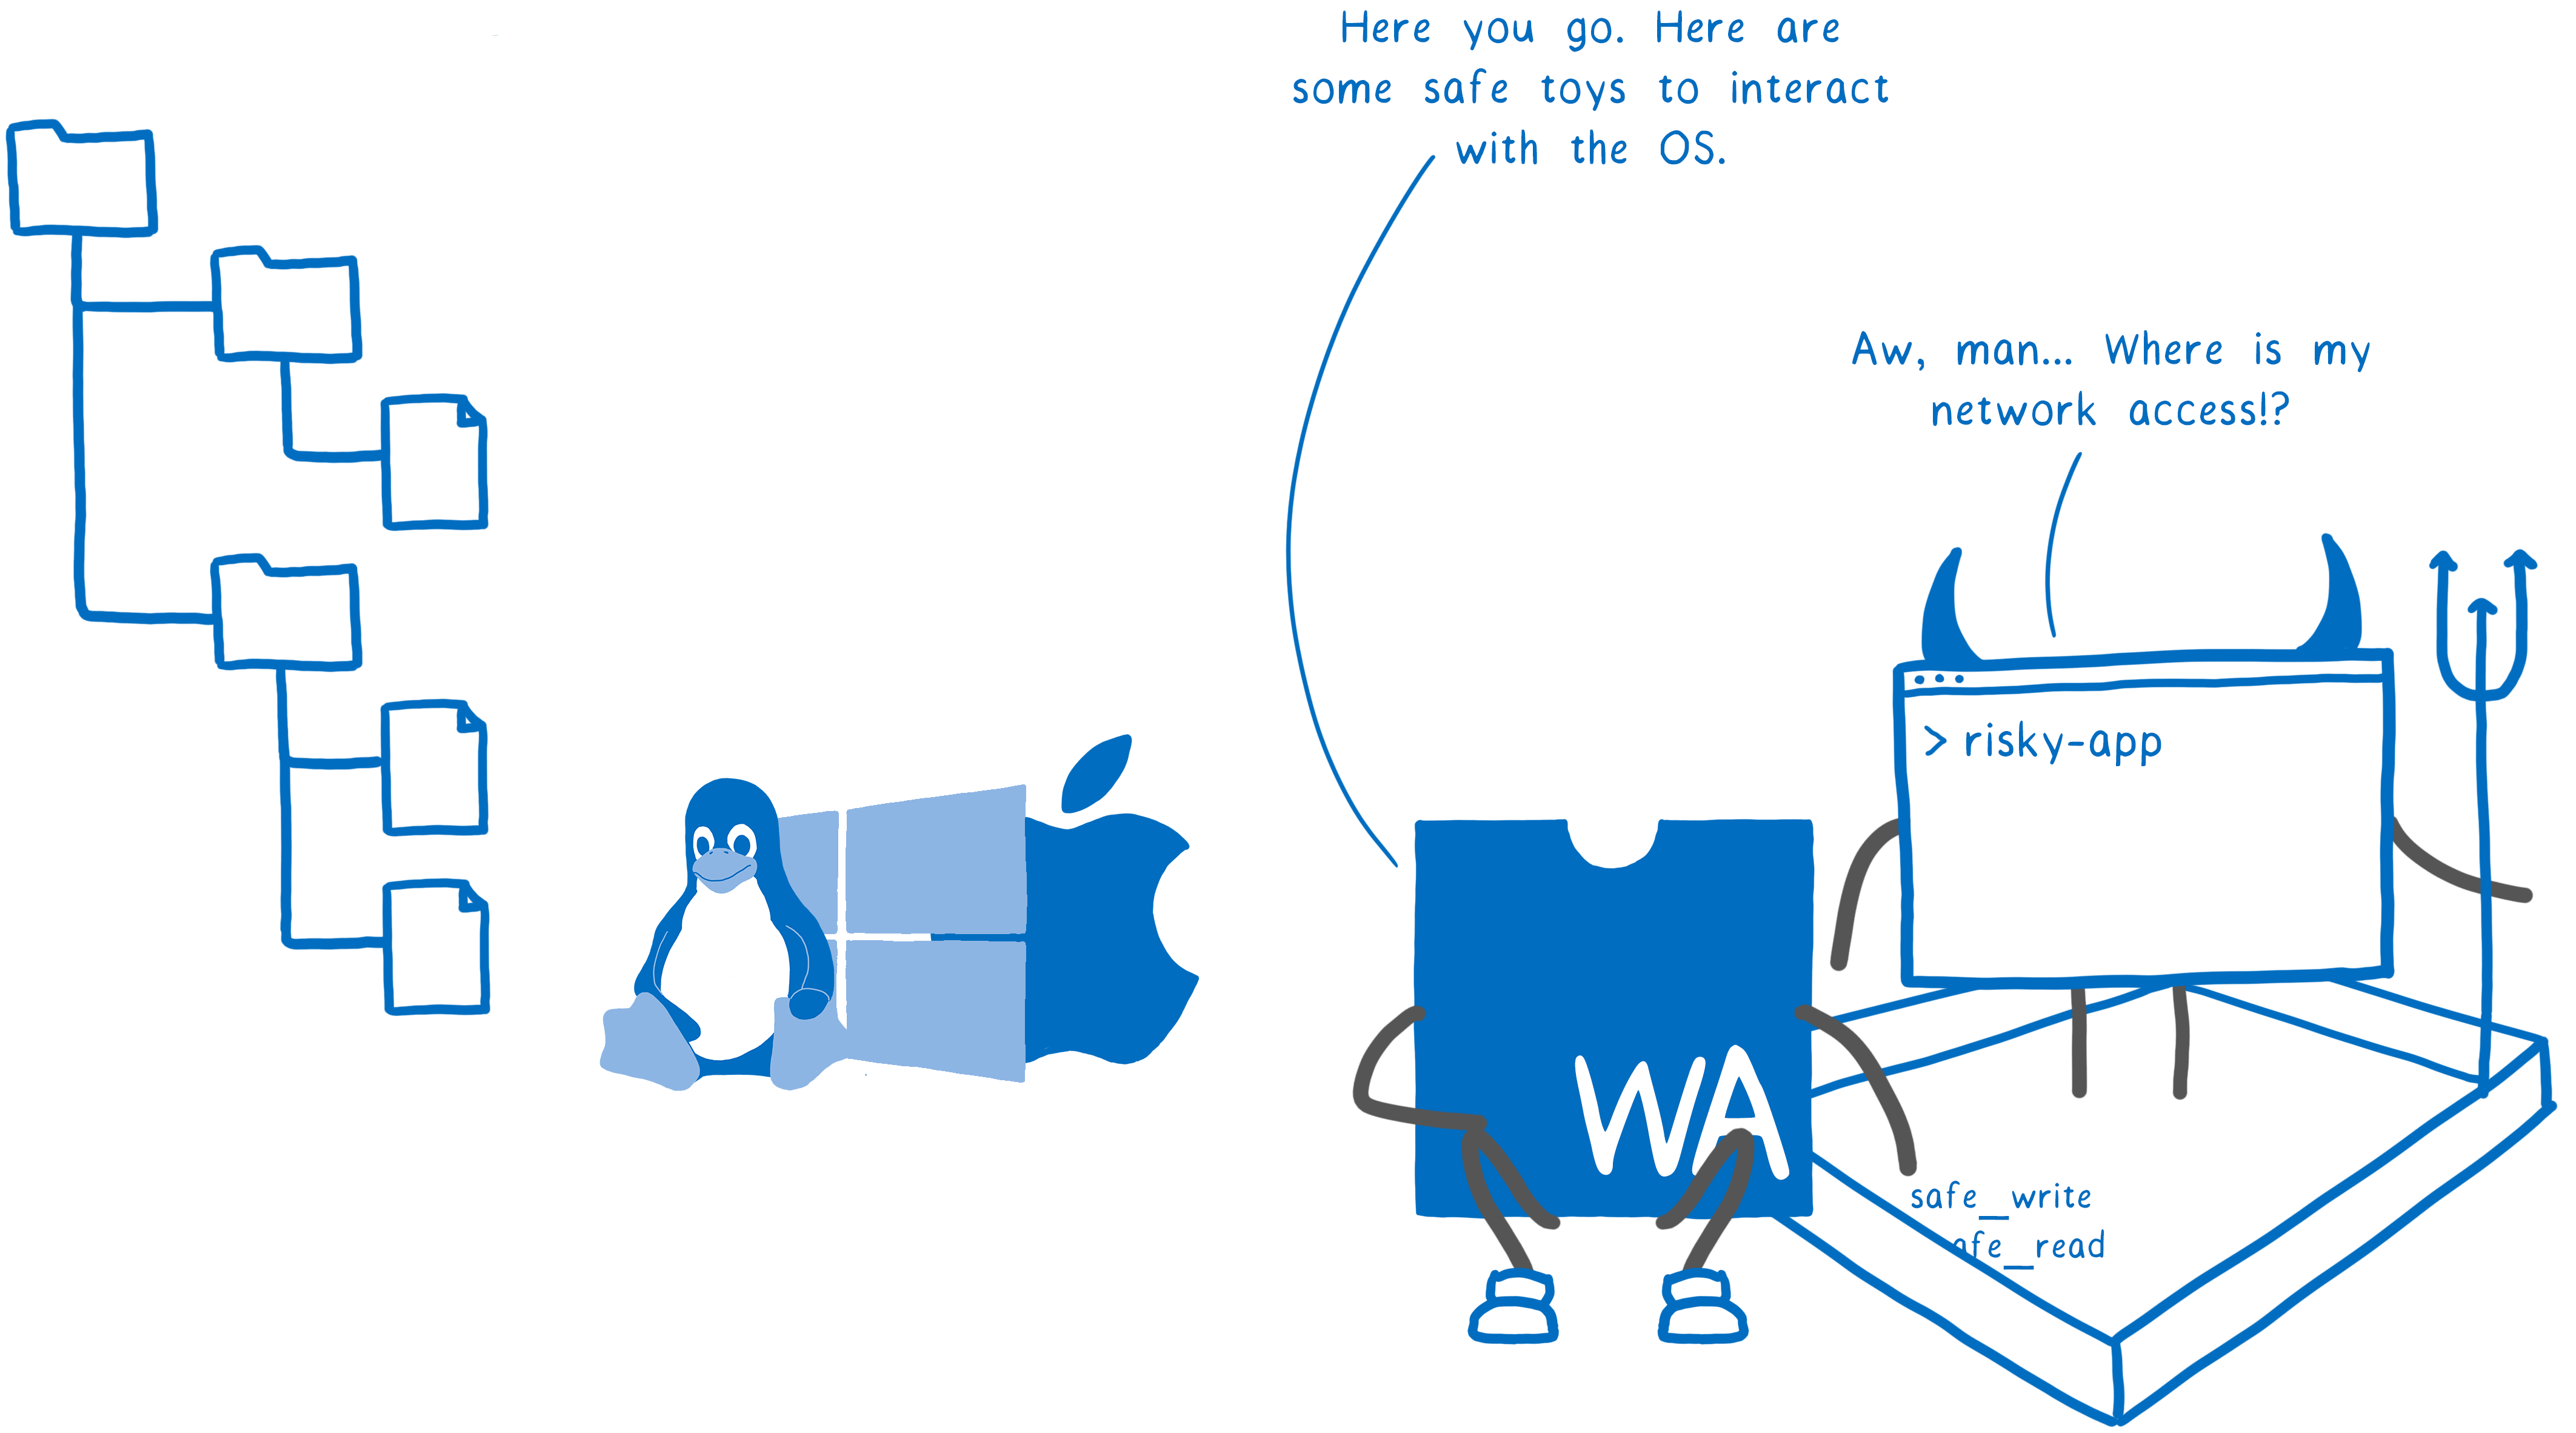
\includegraphics[scale=0.07]{./images/sandbox.png}
        \caption{\href{https://hacks.mozilla.org/2019/03/standardizing-wasi-a-webassembly-system-interface/}{Sandboxing}}
    \end{figure}
\end{frame}

% \item In normal OS, if code needs to open file, it calls the open function containing a string with the path to the file. This succeeds if the user has necessary permissions. 
% \item Instead if you call a function interacting with the files in WASI, you have to pass a file descriptor, which has permissions attached to it. This way you can't randomly open a file. Instead the code can only operate in the directory it was given.
% \item So the runtime passes in the file descriptors that an app can use at the top level code. The code itself can then propagate those file descriptors through the rest of the modules needed (Insert cude picture here)
\begin{frame}{WebAssembly System Interface - WASI}
    \begin{figure}
        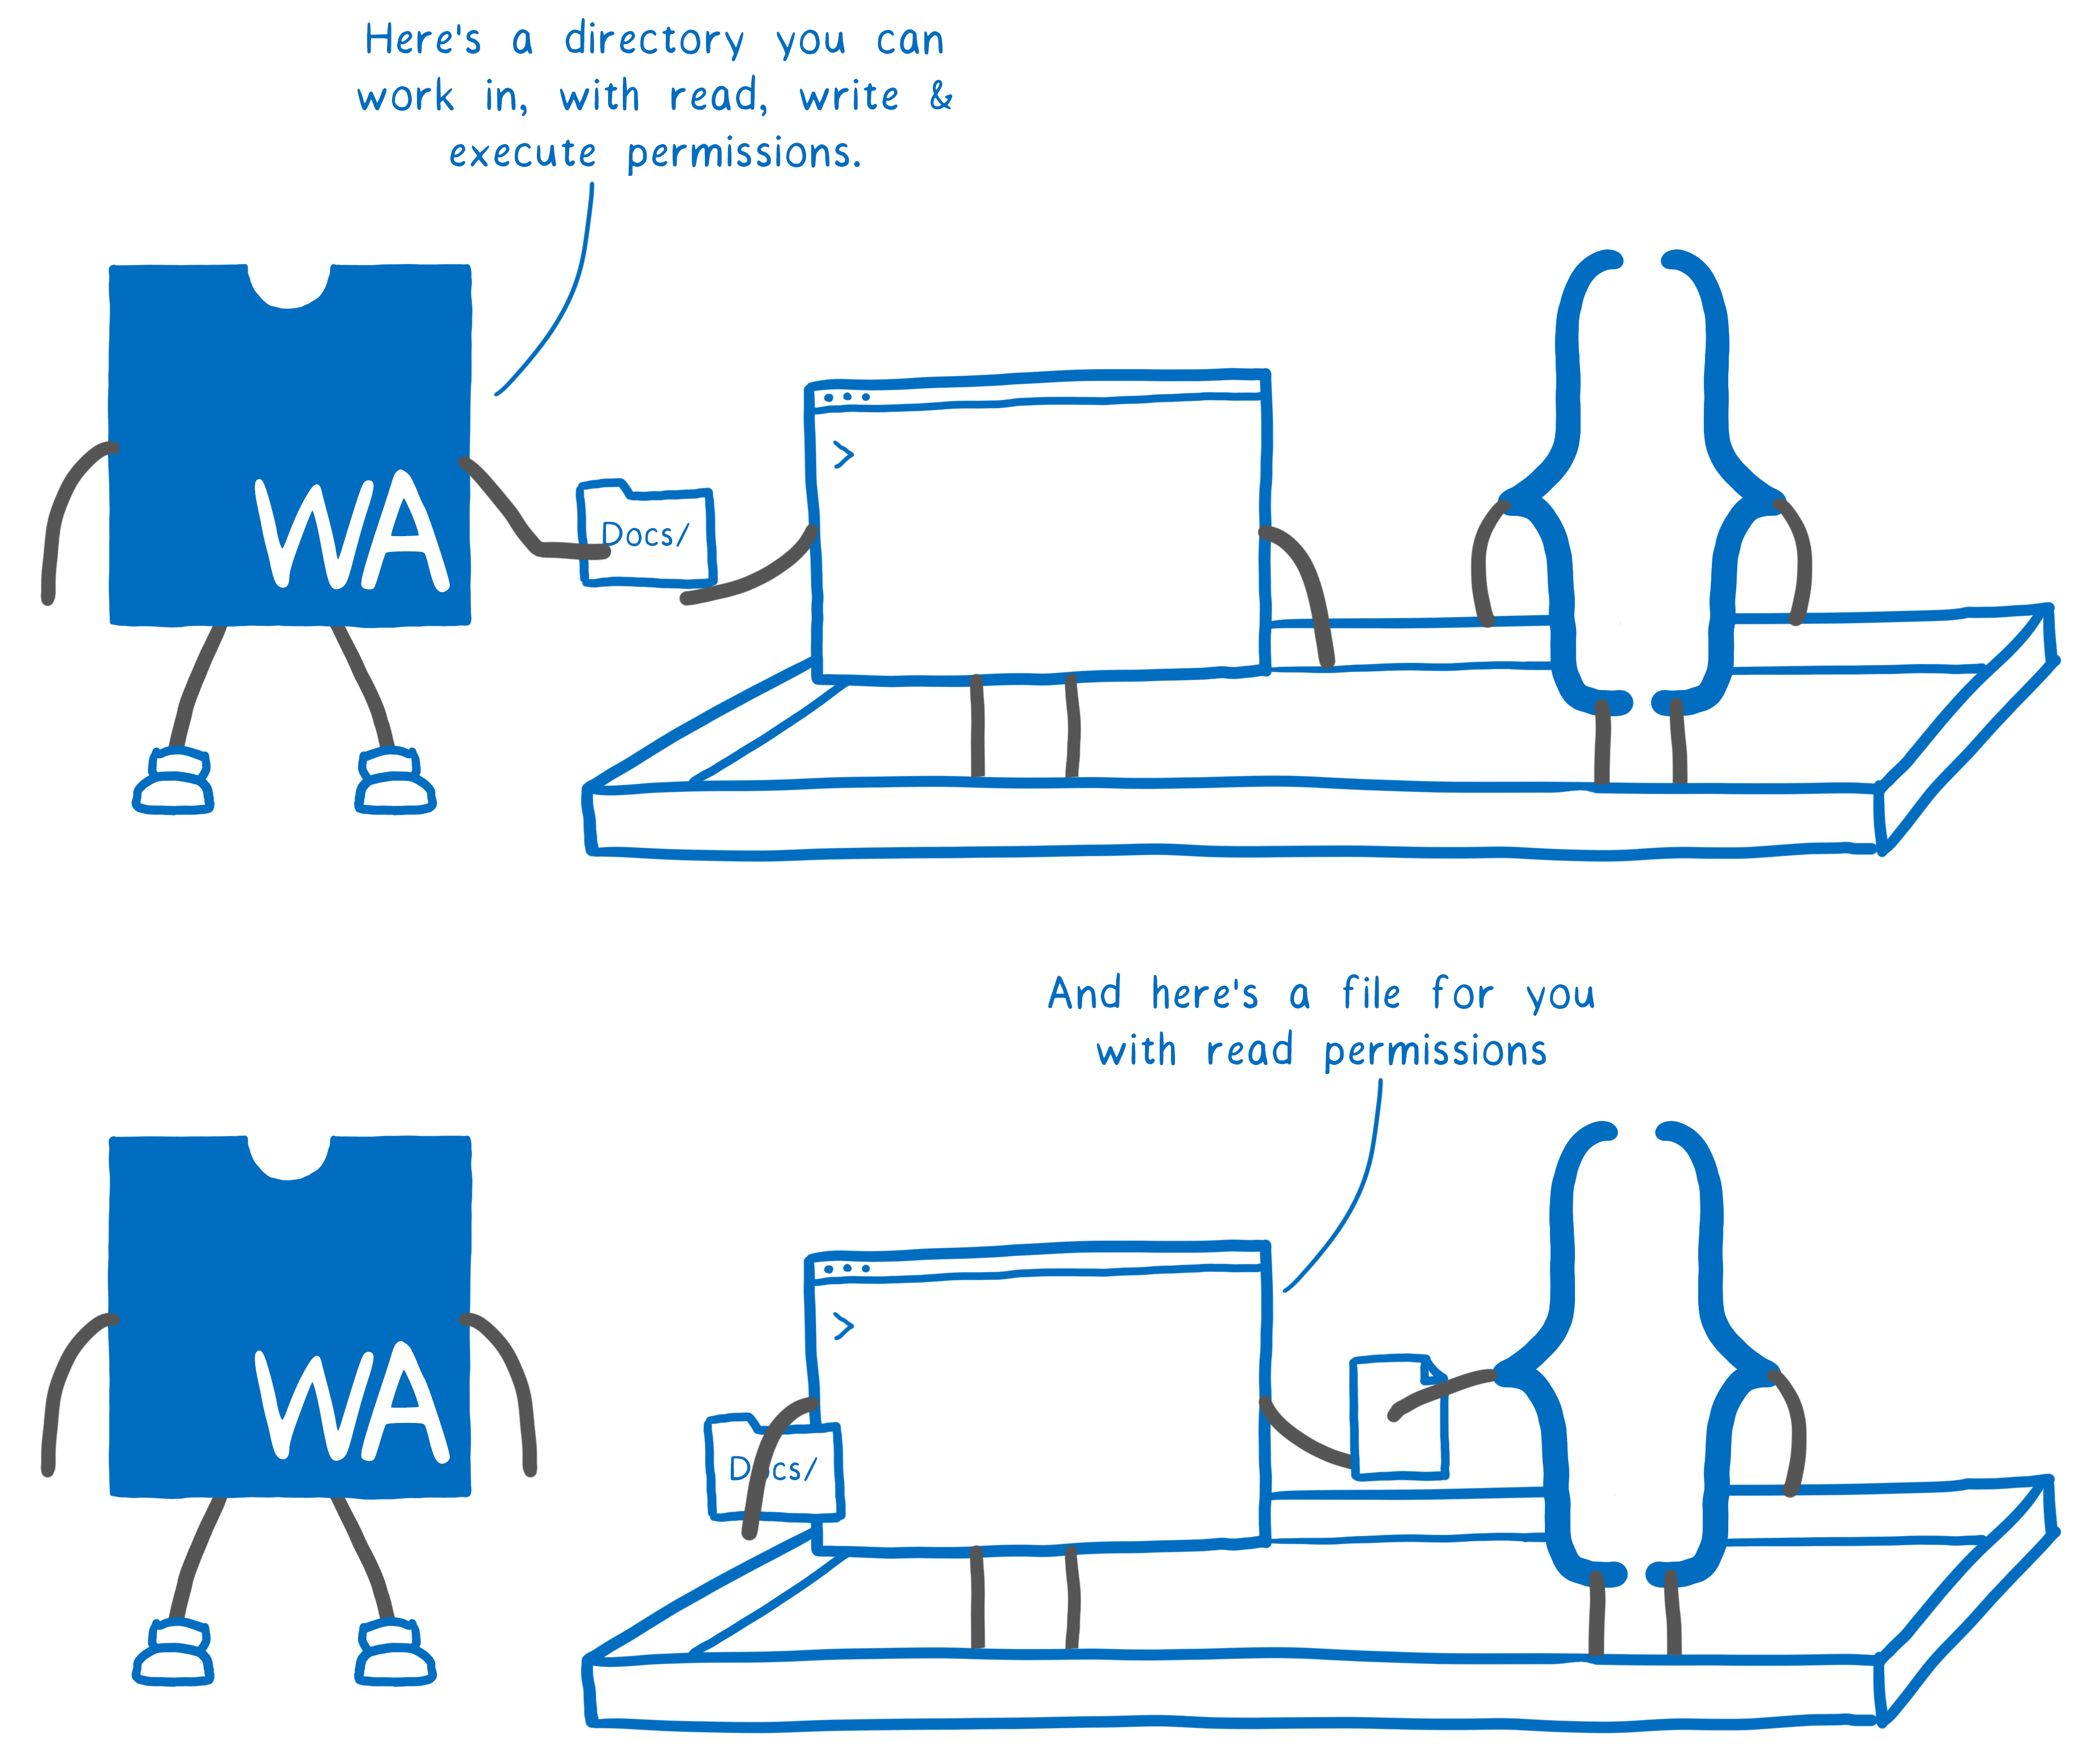
\includegraphics[scale=0.06]{./images/file.png}
        \caption{\href{https://hacks.mozilla.org/2019/03/standardizing-wasi-a-webassembly-system-interface/}{File Descriptor}}
    \end{figure}
\end{frame}

\subsection{WebAssembly Gateway Interface - WAGI}
% WAGI - Read infoq article
\begin{frame}{WebAssembly Gateway Interface - WAGI}
    \begin{itemize}
        \item HTTP handlers using STDIN and STDOUT and environment variables
        \item Write microservices and web apps
        \item Problem this tries to solve: A wasm binary is no server. It is not actively listening. It doesn't even need to run all the time. So how do we get HTTP requests?
        \item When HTTP request is received the WASM binary gets executed with the necessary Information contained in STDIN and environment variables. Replies are sent to STDOUT and binary can terminate again.
        \item WAGI-Server can be used
    \end{itemize}
\end{frame}

\section{Conclusion}

\begin{frame}{Conclusion}
WASM does't have direct access to the DOM, so for all DOM interaction it has to go through JS with a bunch of glue code between. Which means for most normal websites plain JS will be faster than JS + glue code + WASM. If you have some functionality that could really benefit from performance and doesn't just lose it all thorugh foreign function interfaces (FFI) and DOM interaction, then WASM can be really benefitial.
\end{frame}

\begin{frame}{Conclusion}
    \begin{figure}
        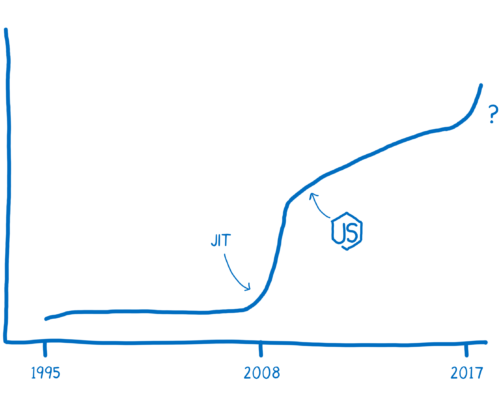
\includegraphics[width=0.7\textwidth,height=0.7\textheight]{./images/perf_history.png}
        \caption{\href{https://hacks.mozilla.org/2017/02/a-cartoon-intro-to-webassembly/}{Performance-Entwicklung im Web-Kontext}}
    \end{figure}
\end{frame}

\begin{frame}{Webshop}

\end{frame}

\end{document}